\chapter{А это что за штука? Устройство гитары}
\label{ch:guitar}

Гитара завоевала сердца многих благодаря простоте и изяществу своего устройства.

Гитара --- это инструмент для извлечения звуков равномерно-темперированного строя. Этот строй уже упоминался в разделе \ref{ch:music}, и сейчас придётся вспомнить его основные особенности.

По сути, строй --- это правила отбора частоты колебаний основного тона для звуков, которые будут называться \emph{музыкальными}. И только такие, и никакие другие, звуки можно извлекать из \emph{музыкального} инструмента.

Из всего диапазона частот звуков, слышимых человеком, нужно отобрать конечное множество <<правильных>>, <<музыкальных>>. В равномерно-темперированном строе это делается так:
\begin{itemize}
    \item Фиксируется частота эталонного звука. Эталонном служит нота ЛЯ первой октавы с частотой 440 Гц. То есть гитарная струна издавая этот звук, будет совершать 440 полных колебаний. Обозначим эту эталонную частоту: $f_{A1}$. Пояснию, что $A1$ --- латинское обозначение для ноты ЛЯ первой октавы.
    
    \item Вводится правило получения частоты $n$-го музыкального звука на основе эталонной частоты. Частота $n$-го музыкального звука $f(n)$ будет определяться так: 
    \[
        f(n) = f_{A1}\cdot{\sqrt[12]{2}}^n,
    \]
    причем $n$ --- число целое, то есть может быть и отрицательным: $\ldots, -2, -1, 0, 1, 2, \ldots$.
\end{itemize}

Пара важных замечаний:
\begin{itemize}
    \item Частоты соседних музыкальных звуков отличаются в $\sqrt[12]{2}$ раз:
    \[
        \frac{f(n+1)}{f(n)} = \frac{f_{A1}\cdot{\sqrt[12]{2}}^(n+1)}{f_{A1}\cdot{\sqrt[12]{2}}^n} = \sqrt[12]{2}.
    \]

    Условную единицу расстояния между соседними звуками, т.е. $n$-м и $(n+1)$-м называют \emph{полутоном}. Это элементарная, неделимая единица расстояния между звуками. 

    \item В равномерно-темперированном строе 12 полутонов составят \emph{октаву} --- условное расстояние, на котором частоты звуков будут отличаться в два раза:
    \[
        \frac{f(n+12)}{f(n)} = \frac{f_{A1}\cdot{\sqrt[12]{2}}^(n+12)}{f_{A1}\cdot{\sqrt[12]{2}}^n} = {\sqrt[12]{2}}^12 = 2.
    \]
    
    Другими словами, равномерно-темперированный строй <<делит>> \emph{октаву} на 12 \emph{полутонов}. Напомню, что в разделе \ref{ch:music} мы разобрались, что если извлечь на реальных струнах звуки, частоты которых отличаются в два раза, то они \emph{идеальным} образом сольются в один звук.
\end{itemize}

Вот и вся, в целом нехитрая, математика равномерно-темперированного строя. Давайте постатаемся её увидеть в конструкции гитары и разберемся с тем, как правильно настроить гитару.


\section{Может разберем? Конструкция}
\label{ch:guitar:construction}

Коснёмся особенностей устройства гитары, которые позволяют извлекать звуки именно такими, какими они должны быть. 

Для начала стоит взглянуть на рисунок \ref{fig:guitar:construction}, чтобы узнать, как называются отдельные части гитары.

\begin{figure}[!ht]
    \centering
    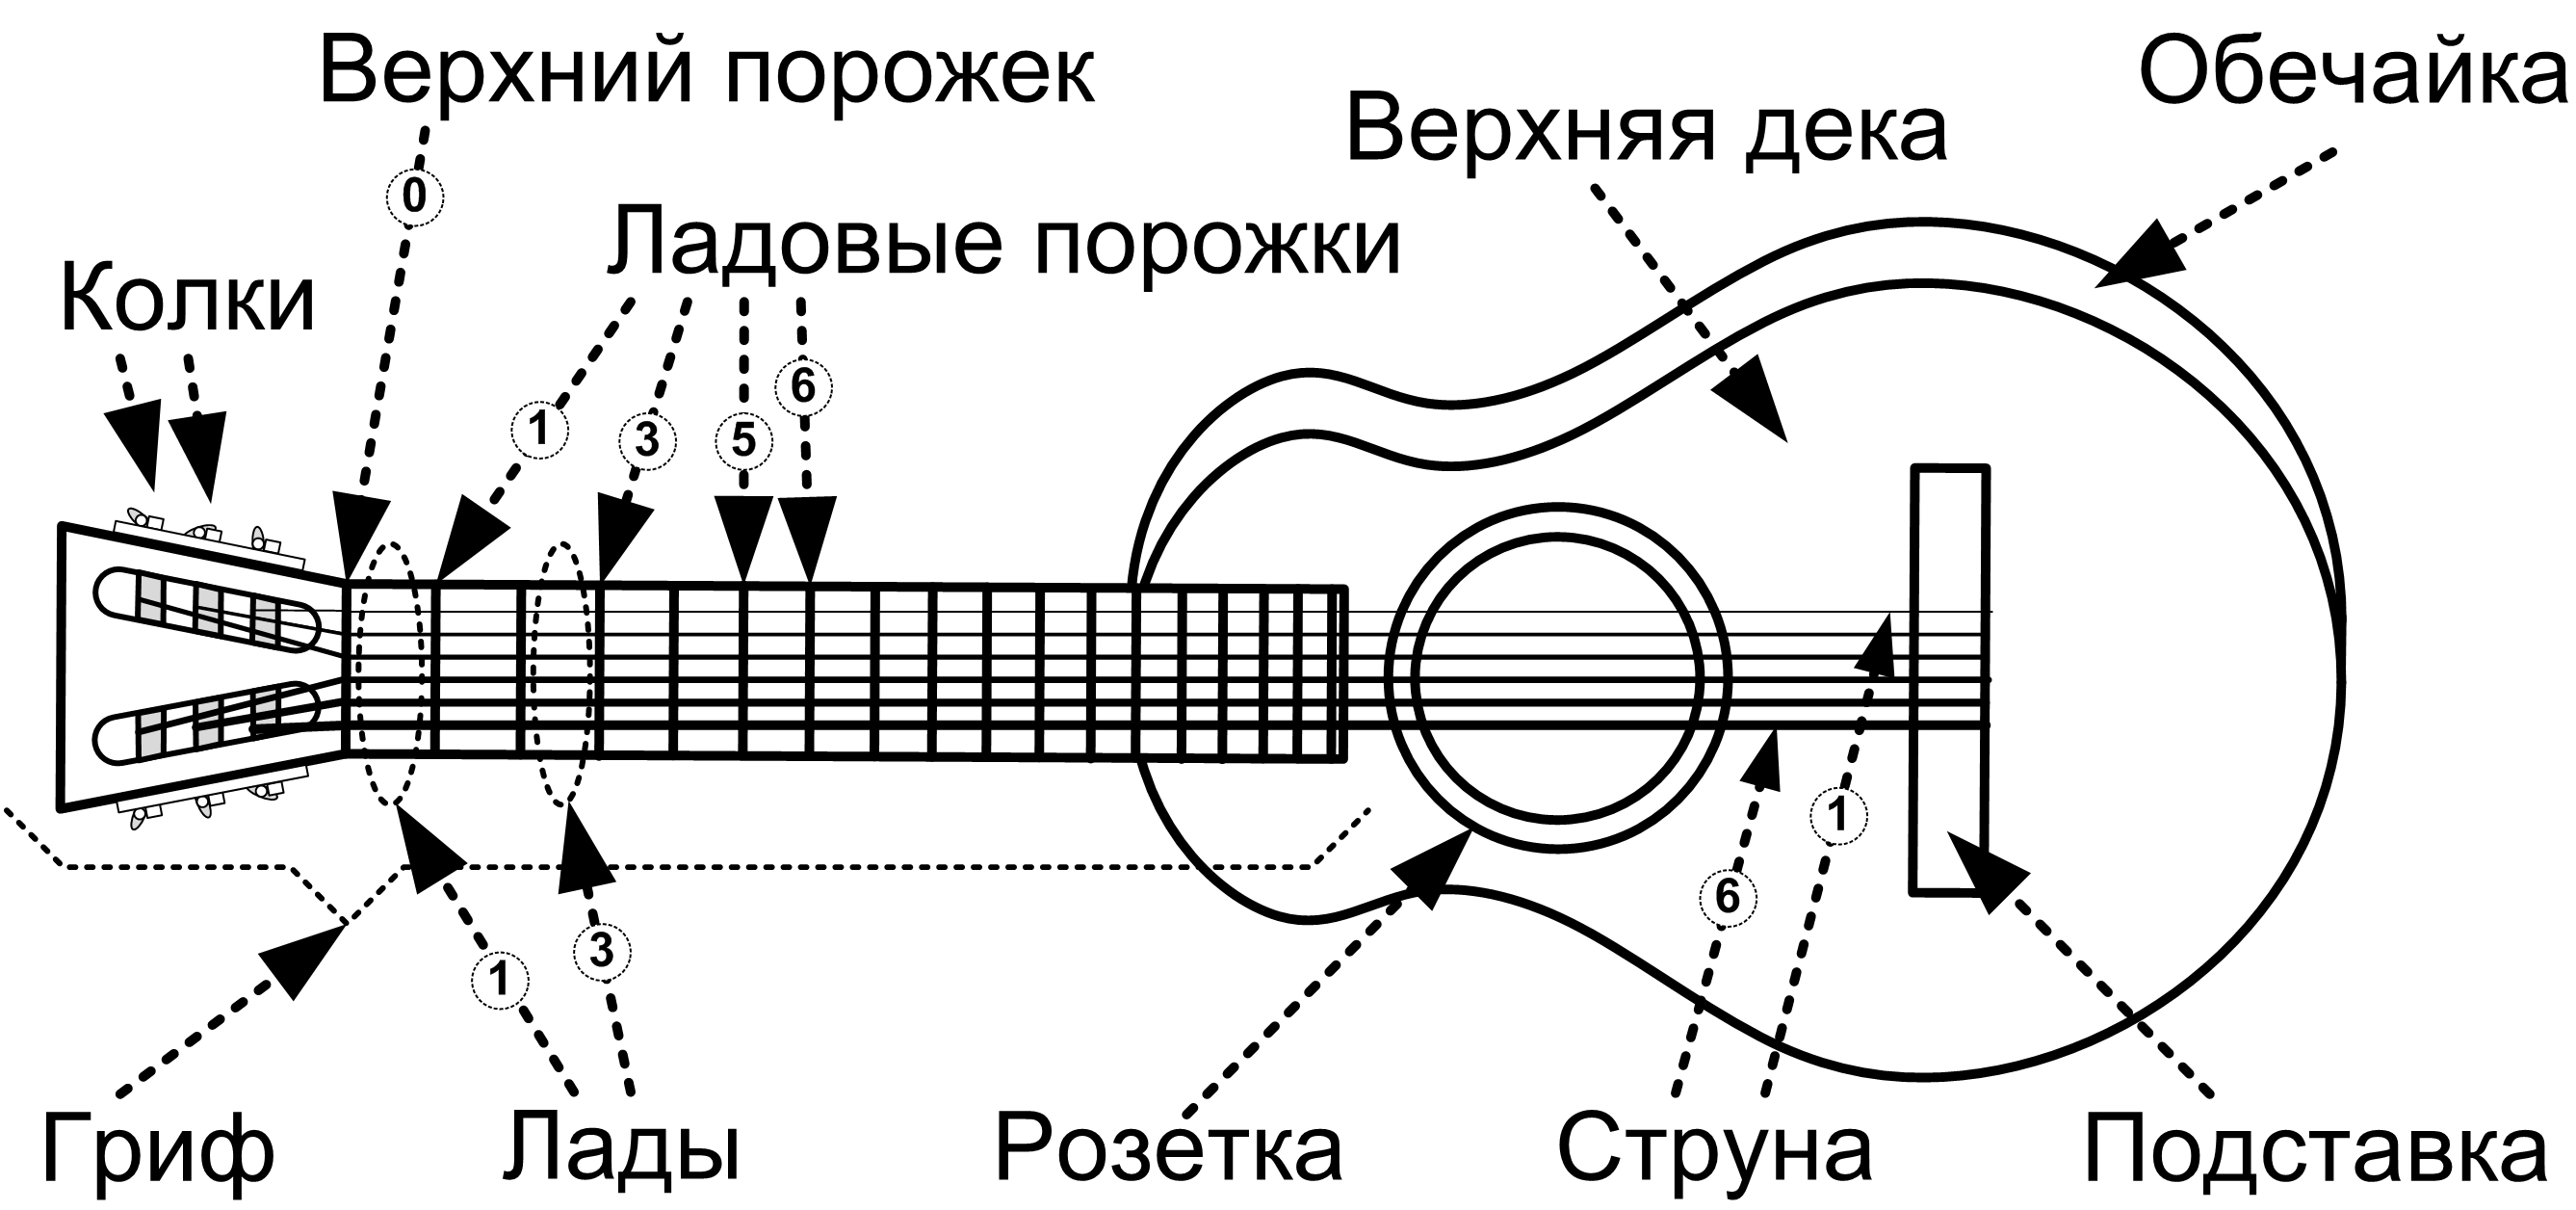
\includegraphics{fig/guitar-construction} 
    \caption{Устройство гитары}\label{fig:guitar:construction}
\end{figure} 

Любая открытая\footnote{То есть не зажатая ни на каком ладу} струна гитары звучит строго определенной нотой (о настройке гитары поговорим позже). Лады на грифе (промежутки между порожками), равно как и \emph{ладовые порожки} считаются от \emph{верхнего} порожка: 1,2,3,\ldots и т.д. То есть <<зажать струну на первом ладу>> значит, что вы ставите палец на струну, на первый лад, то есть между верхним порожком и первым ладовым\footnote{Чем ближе к первому ладовому, тем лучше. Таким образом и звук будет чище, и рука уставать будет меньше. Ставить палец сверху на порожек не стоит --- звук будет <<глохнуть>>. Правда иногда именно это и требуется. Но в начале обучения стоит ставить палец на ладу ближе к тому порожку, от которого идет <<звучащая>> часть струны. Добивайтесь чистого звука.} и нажимаете до тех пор, пока струна не прижмётся к первому ладовому порожку. Но нам важно сейчас не то, как правильно зажимать струну. 

Важно понять, что каждый следующий лад повышает звук на струне на <<полутон>>. В октаве 12 нот и каждая звучит на струне на своём ладу. На дветадцатом ладу звучит нота открытой струны, только выше на октаву.

Из физики известно, что частота колебаний струны обратно пропорциональна её длине\footnote{Надо честно заметить, что частота колебаний струны зависит также и от силы её натяжения, которая меняется, когда струну <<зажимают>> на ладу. Но это влияние столь незначительно, что им можно пренебречь.}. Стало быть, чтобы частота издаваемого струной звука \emph{увеличилась} вдвое (а языком музыки --- чтобы нота зазвучала октавой выше), надо вдвое \emph{укоротить} струну. 

Зажимая струну на 12 ладу (языком музыки --- повышая ноту открытой струны на октаву), вы укарачиваете звучащую часть струны вдвое. Линейка в помощь, если не верите\footnote{Конечно нужно мерять только звучащую (колеблющуюся часть) струны от опоры на подставке до 12-го ладового порожка.}.

Конечно, частота колебаний струны зависит также и от силы её натяжения. Сила натяжения струны регулируется колками на грифе, когда гитару настраивают. Играя, гитарист только меняет длину звучащего участка струны, зажимая струны на ладах. Редкие психи\footnote{Конечно, имелось в виду: \emph{мастера}! Прим. ред.} крутят колок во время исполнения, добиваясь сомнительных\footnote{Конечно, имелось в виду: \emph{удивительных}! Прим. ред.} эффектов.

Исходя из того, что частота каждой следующей ноты в $\sqrt[12]{2}$ больше предыдущей, запишем формулу длины струны ($L$) от места крепления струны к подставке до $n$-го ладового порожка:

\begin{equation}
    \label{fig:guitar:construction:length}
    L(n)=\frac{L}{(\sqrt[12]{2})^n},
\end{equation}

где $n$ - номер лада ($0$-й лад соответствует открытой струне), а $L$ --- общая длина струны от подставки до верхнего порожка.


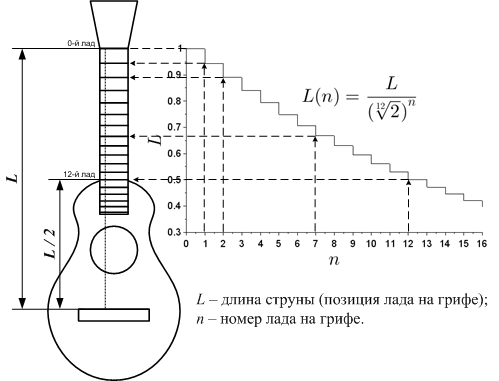
\includegraphics{fig/string-length.png}


Из картинки, надеюсь, ясно, почему ладовые порожки на гитаре расположены не на равном расстоянии друг от друга.

Кстати, некоторые ушастые выпендрёжники говорят, что различают своим сверхмузыкальным слухом больше 12 нот в октаве! И им мало 12 ладов! Есть спрос --- есть предложение: на некоторых гитарах можно заметить дополнительные ладовые порожки между <<каноническими>>, которые позволяют <<всунуть>> дополнительную ноту.


\section{Правильно устроена? --- не значит что настроена!}
\label{ch:guitar:tuning}

\begin{figure}[!ht]
    \centering
    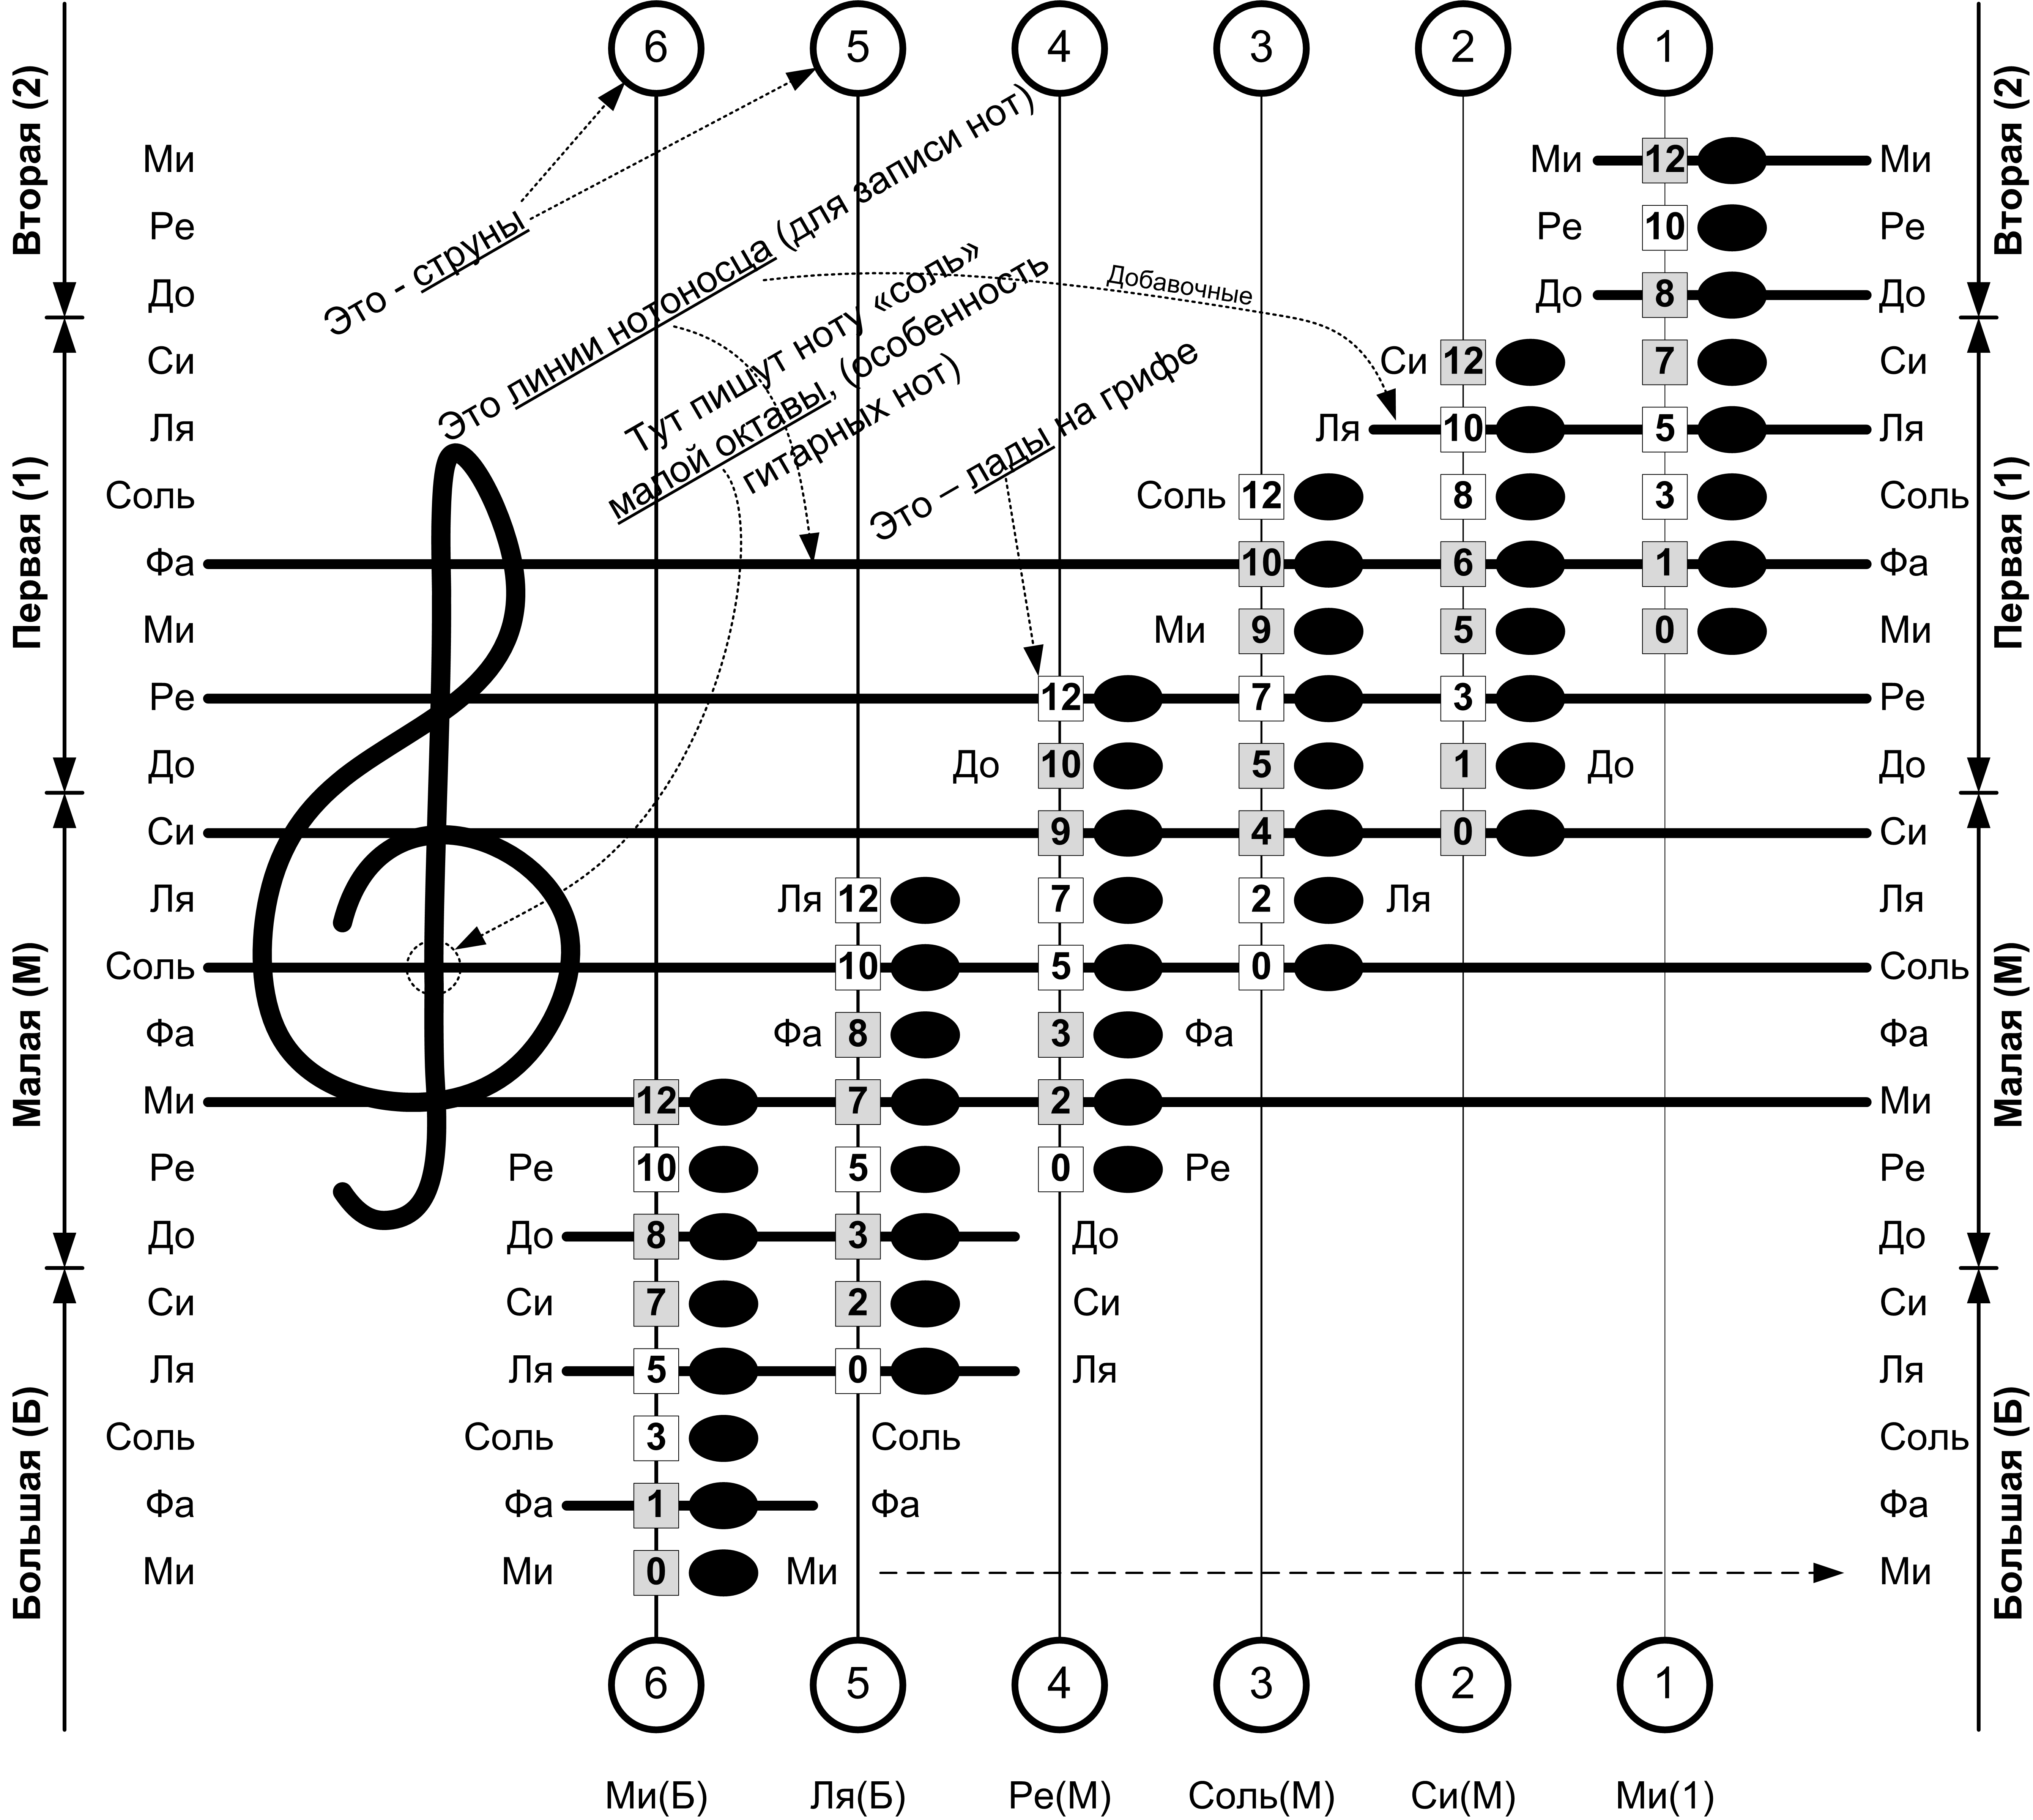
\includegraphics[width=\textwidth]{fig/lad-by-notes} 
    \caption{Ноты на грифе (гриф поперек нотоносца)}\label{fig:guitar:lad-by-notes}
\end{figure} 

\begin{figure}[!ht]
    \centering
    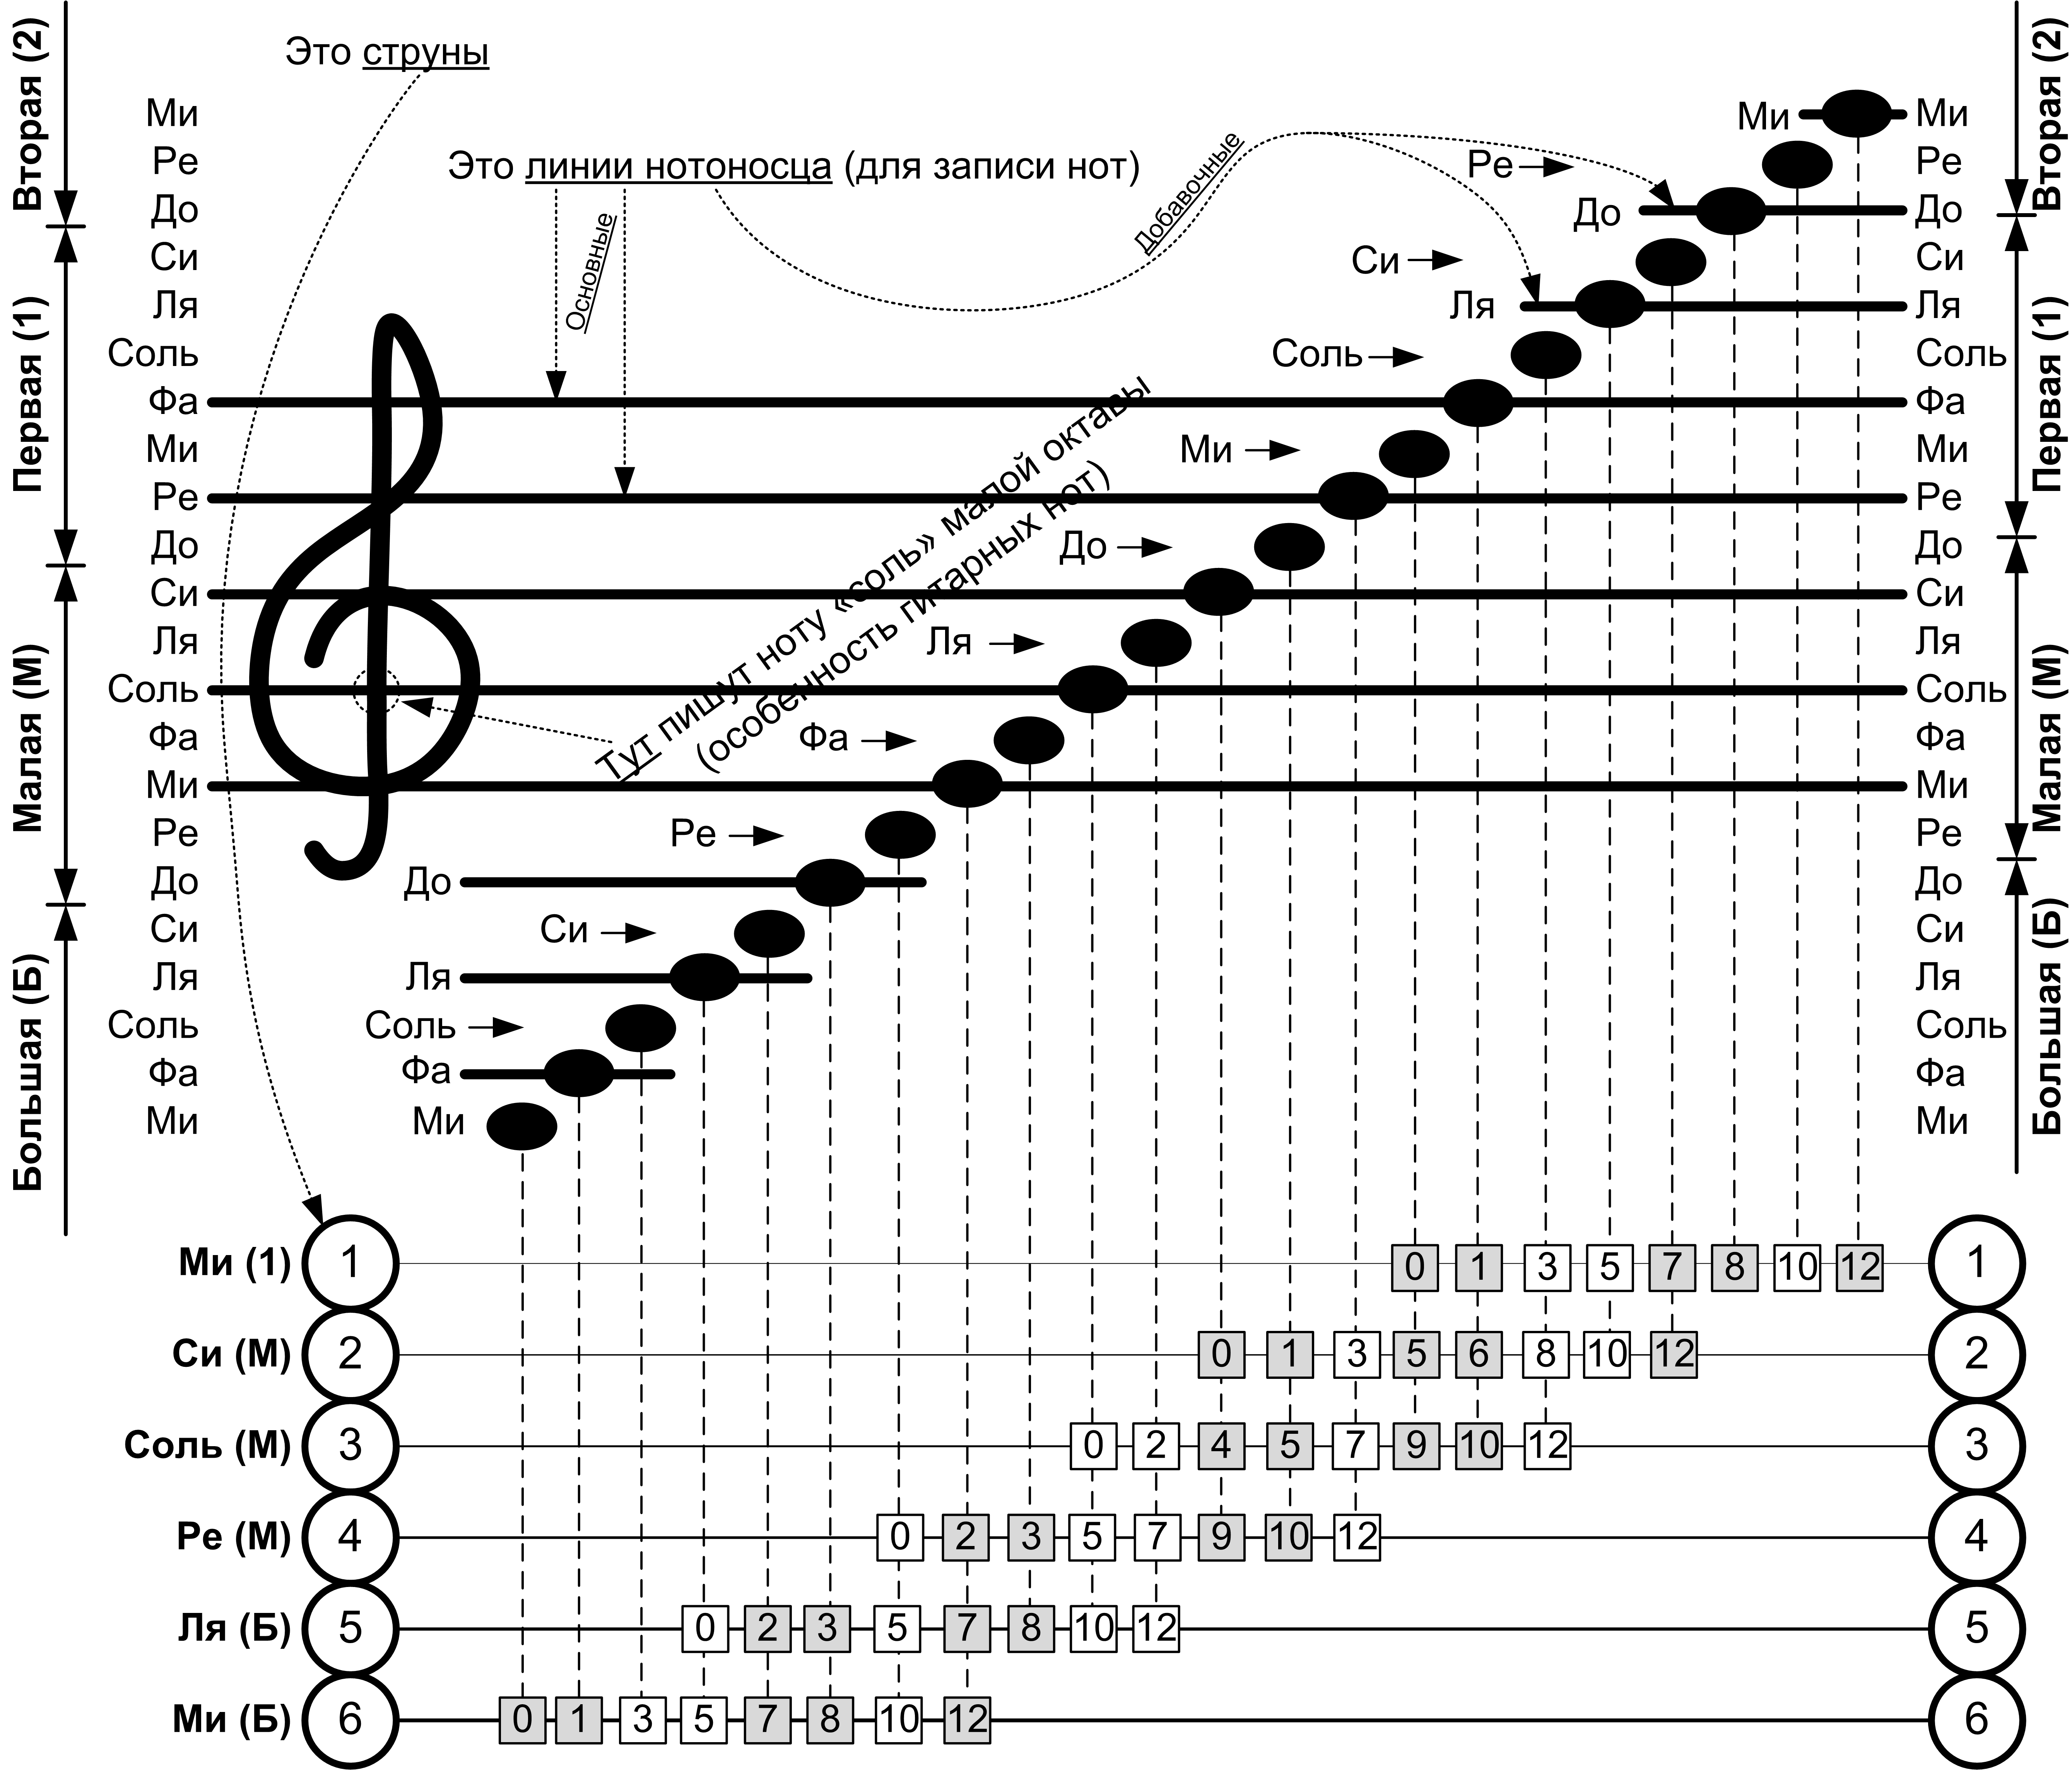
\includegraphics[width=\textwidth]{fig/lad-by-griph} 
    \caption{Ноты на грифе (гриф вдоль нотоносца)}\label{fig:guitar:lad-by-griph}
\end{figure} 

\begin{figure}[!ht]
    \centering
    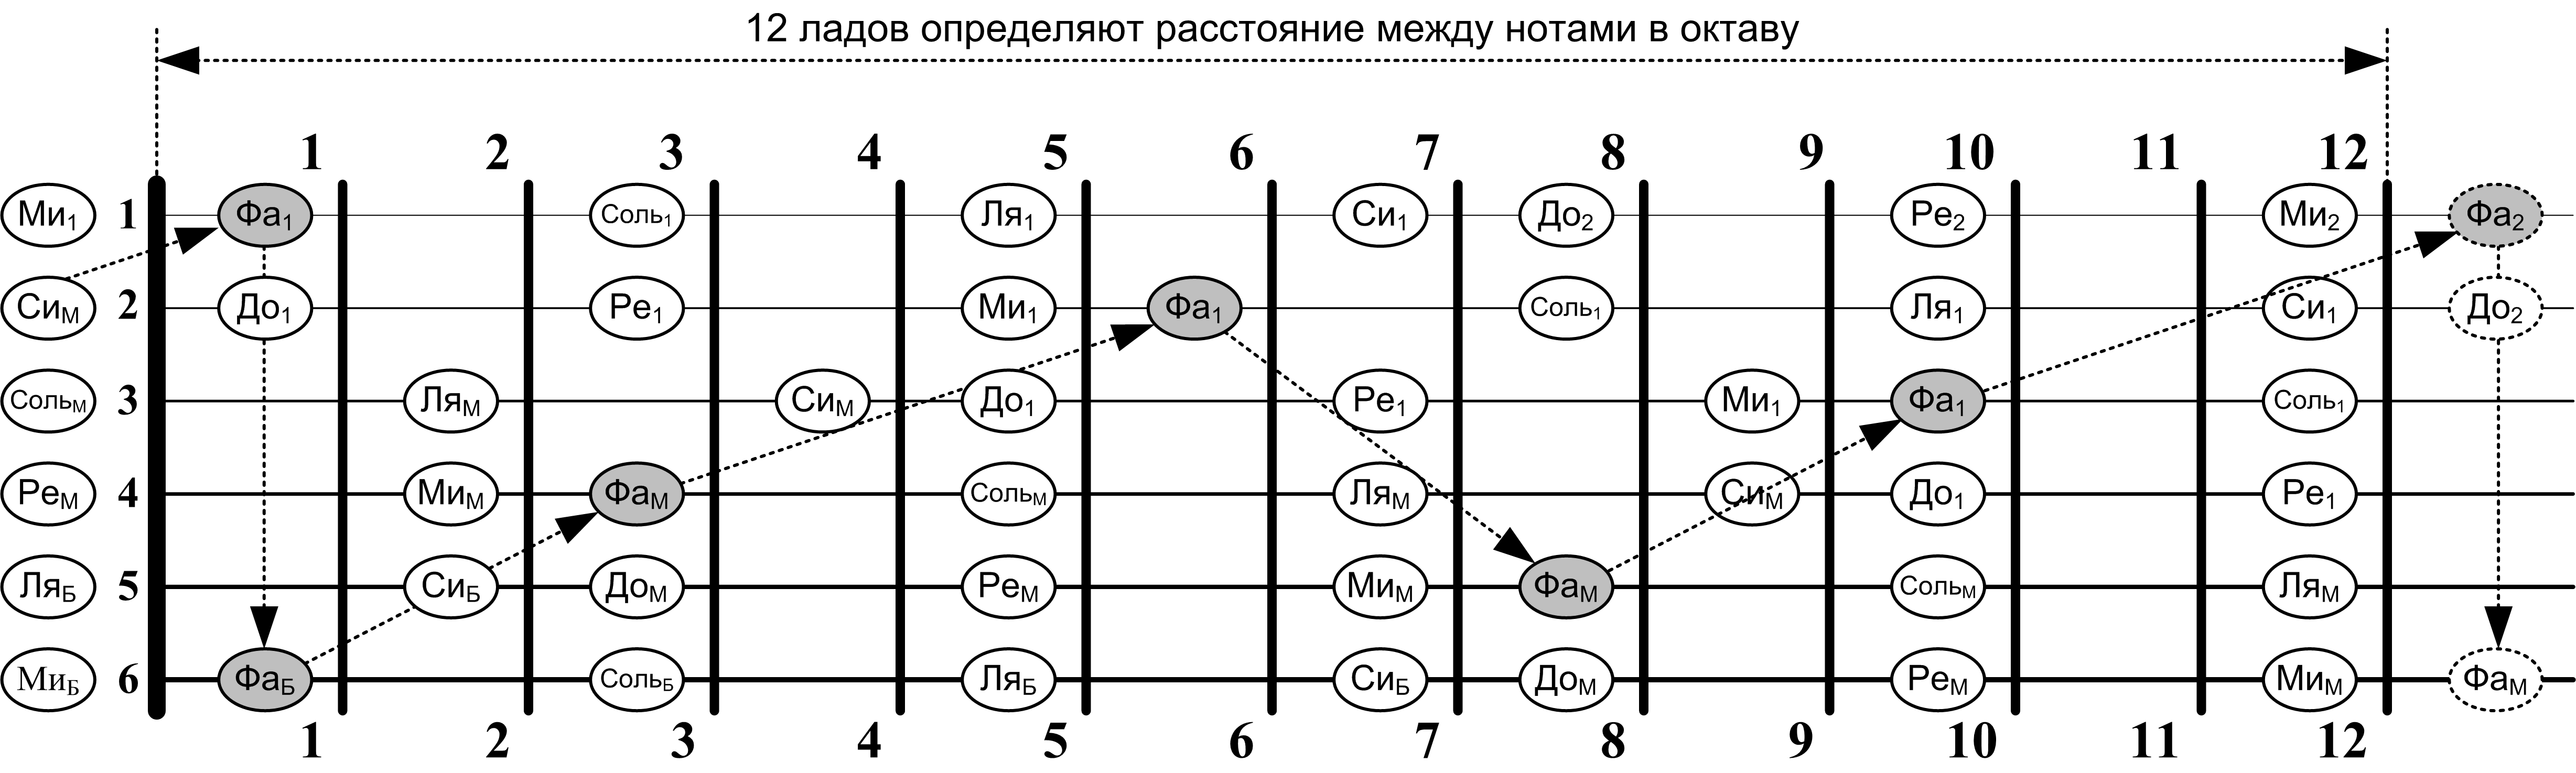
\includegraphics[width=\textwidth]{fig/notes-on-griph} 
    \caption{Ноты на грифе (относительное расположение)}\label{fig:guitar:notes-on-griph}
\end{figure} 


